\documentclass[defense.tex]{subfiles}
\begin{document}




\begin{frame}{}

\centering\Huge {\color{darkred}\textbf {Part II}}:\\
Accelerating Convolutional\\Sparse Coding\\
\biblio{}
	
\end{frame}

%-----------------------------------------------------------------------------

%-----------------------------------------------------------------------------
\section{Convolutional Dictionary Learning}


\begin{frame}{Motivation}

	\centering
	\includegraphics[width=.9\textwidth]{CSC}

\end{frame}


%\begin{frame}{Dictionary Learning for Time Series}
%
%	\Large
%	{\bf Convolutional dictionary learning}\\[2em]
%
%	\begin{itemize}\itemindent2em\itemsep1em
%		\item Shift invariant patterns
%		\item Separation between the localization and the\\
%		\hskip2em shapes of the patterns
%	\end{itemize}
%\end{frame}


\begin{frame}{Convolutional Sparse Coding}

	For a signal $X$, find the coding signal $Z$ given a set of $K$ patterns $\pmb D$.

	\vskip.6em
	\begin{block}{Optimization problem}
	Solve a $\ell_1$-regularized minimization problem
	\begin{equation}\label{eq:sparse_code}
		Z^* = \arg\min_{Z} E(Z) = \frac{1}{2} \|X - \sum_{k=1}^KZ_k*\pmb D_k\|_2^2 + \lambda\|Z\|_1,
	\end{equation}
	\end{block}

	\vskip.5em
	Existing algorithms do not scale well with the size of the signal $X$.\\[1em]

	\begin{itemize}\itemindent1em
		\item Feature Sign Search (FSS) \mycite{Grosse2007}
		\item Fast Iterative Soft Thresholding (FISTA) \mycite{Chalasani2013}
		\item Fast Convolutional Sparse Coding (FCSC) \mycite{Bristow2013}
		\item Coordinate Descent (CD)  \mycite{Kavukcuoglu2013}
	\end{itemize}

\end{frame}

\begin{frame}{Coordinate Descent (CD)}

Update the problem for one coordinate at each iteration.\\
The problem in one coordinate is:
$$
	e_{k, t}(u) = \frac{\|\pmb D_k\|_2^2}{2}\left(u - \beta_k[t]\right)^2 + \lambda |y|
$$
with {\small $\beta_k[t] = \left(\left(X- \Phi_{k, t}(Z)*\pmb D^T\right)* \widetilde {\pmb D}_k\right)[t]$}.\\[.5em]
Three algorithms based on this idea:\\[.5em]
\begin{itemize}\itemindent2em
	\item Cyclic updates \mycite{Friedman2007}
	\item Random updates \mycite{Nesterov2010}
	\item Greedy updates \mycite{Osher2009}
\end{itemize}
\vskip1em
Recent work shows it is more efficient to use greedy updates.\\\mycite{Nutini}

\end{frame}


\begin{frame}{Convolutional Coordinate Descent}

For convolutional CD, we can use greedy updates:
$$
	Z'_k = \frac{1}{\|\pmb D_k\|_2^2}\text{Sh}(\beta_k, \lambda),
$$
with {\small $\text{Sh}(y, \lambda) = \text{sign}(y)(|y| - \lambda)_+$}.\\[2em]
This can be done efficiently for this problem  by maintaining $\beta$, with $\mathcal O(KS)$ operations. 	\mycite{Kavukcuoglu2013}

$$
\beta_k^{(q+1)}[t] = \beta_k^{(q)}[t] - \mathcal S_{k, k_0}[t-t_0] (Z_{k_0}[t_0]-Z'_{k_0}[t_0]),
$$\\[1em]
with $\smeq\mathcal S_{k, k_0}[t] = \sum_{\tau=0}^{S-1}\pmb D_{k}[t+\tau] \pmb D_{k_0}^T[\tau] $.\\[1em]
\end{frame}


\begin{frame}{Improving Convolutional Coordinate Descent(1/2)}

This is not so efficient to only change one coordinate as updates only affect a small range of coefficients.\\[.5em]
We could update $M$ coefficients that are in disjoint neighborhoods in {\bf parallel}.\\[1.5em]

{\bf Issue: }Choose disjoint coordinates\\
Split the signal in $M$ continuous chunks and perform updates:\\[.5em]
\begin{itemize}\itemindent4em\itemsep.5em
	\item Use a lock to avoid updates that are too close,
	\item Use a parameter server to reject multiple updates.
\end{itemize}
\mycite{Scherrer2012, Bradley2011}
\\\mycite{Yu2012, Low2012}

\vskip1.5em
{\bf Is it necessary?}
\end{frame}

\begin{frame}{Improving Convolutional Coordinate Descent (2/2)}

	Consider the cost function $E(Z) = \frac{1}{2}\|X - \sum_{k=1}^KZ_k*\pmb D_k\|_2^2 + \lambda\|Z\|_1$\\[.5em]

	We denote $\Delta E_0 = E(Z^{(q+1)}) - E (Z^{(q)})$ the update performed at step $q$ for coefficient $(k_0, t_0)$.\\[1em]
	
If we update simultaneously $(k_0, t_0)$ and $(k_1, t_1)$ coefficients, it can be shown that:
$$
\Delta E_{0, 1} = \underbrace{\Delta E_0 + \Delta E_1}_{\text{iterative steps}}
	- \underbrace{\mathcal S_{k_0, k_1}[t_1 - t_0] \Delta Z_0 \Delta Z_1}_{\text{interference}},
$$
\vskip.5em
If interference are not too high, the updates can be asynchronous.
\end{frame}

\begin{frame}{Distributed Convolutional Coordinate Descent (DICOD)}

Each core is responsible for the updates of a chunk of coefficients.\\
\vskip2em

\inputTikZ{1}{dcp_tikz.tex}

\vskip2em
Retrieve the notification when possible to update $\beta$.
\end{frame}

%\begin{frame}{Convergence Analysis}
%We denote:
%$$
%C_{k_0k_1}[t_0-t_1]= \frac{\mathcal S_{k_0, k_1}[t_0-t_1]}{\|\pmb D_{k_0}\|_2\|\pmb D_{k_1}\|_2}.
%$$
%\begin{block}{Theorem}
%We consider the following assumptions:\\[.3em]
%{\bf H1: }
%If for all $k_0, k_1, t_0, t_1$ such that $t_0 - t_1 \neq 0$,  $|C_{k_0k_1}[t_0-t_1]| < 1$.\\[.3em]
%{\bf H2: }
%If there exist $A \in \mathbb N^*$ such that for all $m \in \left \{ 1, \dots M\right \}$ and $q\in \mathbb N$, $\mathcal C_m$ is updated at least once between iteration $q$ and $q + A$ if the solution is not optimal for all coefficients assigned to $\mathcal C_m$.\\[1em]
%Under these assumptions, the DICOD algorithm converges to the optimal solution $Z^*$ of \mbox{\autoref{eq:sparse_code}}.
%\end{block}

%\end{frame}

\begin{frame}{Numerical convergence}
	Generated problems with $\pmb D$ gaussian and $Z$ Bernouilli-Gaussian
	$$
		X = \sum_{k=1}^KZ_k*\pmb D_k + \epsilon
	$$
	\centering
	\only<1>{
		\includegraphics[width=.8\textwidth]{dicod/cost_iter}\\
		Cost as a function of the iterations
	}
	\only<2>{
		\includegraphics[width=.8\textwidth]{dicod/cost_time}\\
		Cost as a function of the time
	}
\end{frame}

\begin{frame}{Complexity Analysis}
	Computational cost of one update for greedy CD is linear in $\mathcal O(T)$:\\[1em]
	\begin{itemize}\itemindent2em\itemsep.5em
	\item Compute potential updates $Z'_k[t]$,
	\item Find $(k_0, t_0) = \arg\min_{k, t} |Z'_k[t] - Z_k[t]|$.
\end{itemize}
\vskip2em
Computational cost for one update of DICOD is linear in $\mathcal O(\frac{T}{M})$:\\[1em]
\begin{itemize}\itemindent2em\itemsep.5em
	\item Same steps but with a signal of size $\frac{T}{M}$.
\end{itemize}
\end{frame}

\begin{frame}{Speedup}
With an analysis of the interference probability, the convergence rate of DICOD with $M$ cores can be bounded by:
\begin{equation}
	\label{eq:seedup}
	\begin{split}
		\mathbb E[S_{dicod}] & \underset{\phantom{\alpha \to 0}}{\ge} \smeq M^2 ( 1- 2\alpha^2M^2\left(\smeq1 +2\alpha^2M^2\right)^{\frac{M}{2}-1})~,\\
		&\smeq\underset{\alpha \to 0}{\gtrsim} M^2(1-2\alpha^2M^2 + \mathcal O(\alpha^4M^4))~.
	\end{split}
\end{equation}
with $\alpha^2 = \left(\frac{SM}{T}\right)^2$ the probability of interference.\\[.5em]
\begin{itemize}
	\item For $\alpha$ close to 0, the speedup is quadratic.
	\item There is a sharp transition as $\alpha$ grows that degrade the performance of the algorithm.
\end{itemize}
\end{frame}


\begin{frame}{Numerical Speedup}

\centering
		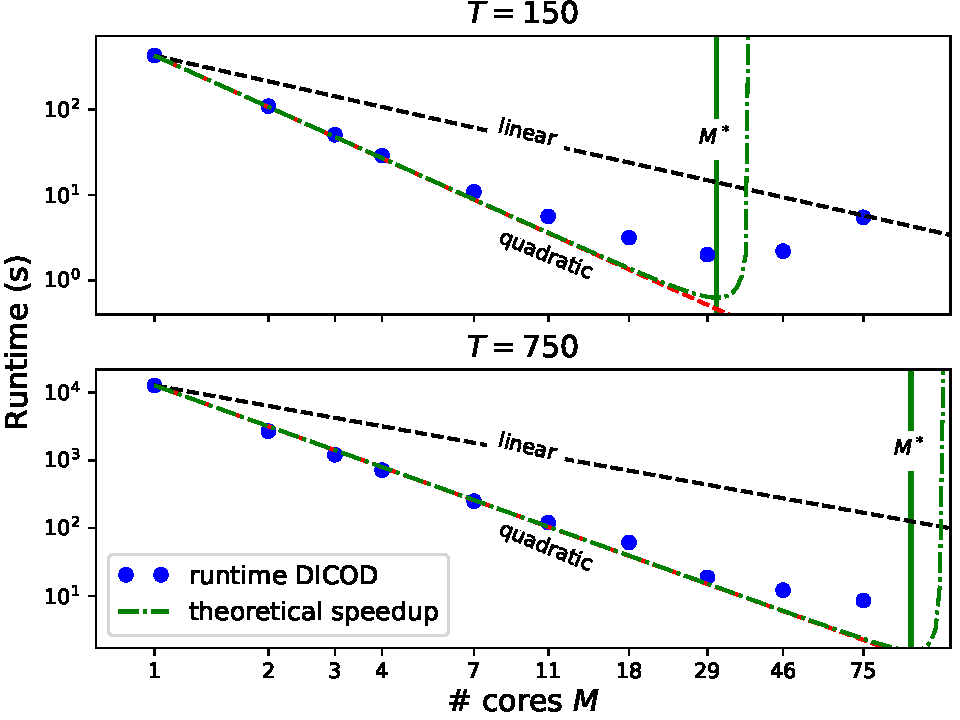
\includegraphics[width=.8\textwidth]{scaling}\\
Runtime as a function of the number of cores

\end{frame}

\begin{frame}{Contributions}
	\textbf{Contributions}
	\begin{itemize}\itemsep.5em
		\item Distributed algorithm efficient to solve the CSC problem
		\item Guaranteed convergence to the optimal solution
		\item Super-linear speedup
	\end{itemize}
	\vskip1.5em
	\textbf{Future work}
	\begin{itemize}\itemsep.5em
		\item Extend this work to 2D case
		\item Handle local penalties
	\end{itemize}
\end{frame}


\end{document}